\documentclass[letterpaper, 10 pt,onecolumn]{article}

\usepackage[papersize={8.5in,11.in},text={7.5in,9.75in}]{geometry}

\usepackage{graphics}
\usepackage{graphicx} % For including and formatting image files
\usepackage{multirow}
\usepackage{longtable}
\usepackage{epsfig}
\usepackage{epstopdf}

\usepackage{amsmath, mathrsfs, dsfont}
\usepackage{amssymb}
\usepackage{amsfonts}
\usepackage{bm}


\usepackage{cite}
\usepackage{verbatim}

\usepackage{amscd}
\usepackage{color}
\definecolor{lgray}{gray}{0.6}
\usepackage{rotating}


%\usepackage[font=footnotesize]{caption}
%\usepackage[caption=false,font=footnotesize]{subfig}
\usepackage[font=footnotesize]{subcaption}

\usepackage{mathptmx}
\usepackage[11pt]{moresize}
\usepackage{flushend}
\usepackage[stable]{footmisc}

\usepackage{algorithmicx}
\usepackage{algorithm}
\usepackage{algpascal}
\usepackage{float}
\usepackage{algc}
\usepackage{algcompatible}
\usepackage{algpseudocode}

\renewcommand{\algorithmicrequire}{\textbf{Input:}}  % Use Input in the format of Algorithm  
\renewcommand{\algorithmicensure}{\textbf{Output:}} % Use Output in the format of Algorithm  
\usepackage[vcentermath]{youngtab} % For typesetting Young Tableaux
\usepackage{url}
%\usepackage{breakurl}   
            

%-----------------------------------------%
% Define custom symbols
\newcommand{\BoldA}				{ \mathbf{A} }
\newcommand{\Bolda}				{ \mathbf{a} }
\newcommand{\BoldB}				{ \mathbf{B} }
\newcommand{\Boldb}				{ \mathbf{b} }
\newcommand{\BoldC}				{ \mathbf{C} }
\newcommand{\Boldc}				{ \mathbf{c} }
\newcommand{\BoldD}				{ \mathbf{D} }
\newcommand{\Boldd}				{ \mathbf{d} }
\newcommand{\BoldE}				{ \mathbf{E} }
\newcommand{\Bolde}				{ \mathbf{e} }
\newcommand{\BoldF}				{ \mathbf{F} }
\newcommand{\BoldG}				{ \mathbf{G} }
\newcommand{\g}					{ \mathbf{g} }
\newcommand{\BoldH}				{ \mathbf{H} }
\newcommand{\Boldh}				{ \mathbf{h} }
\newcommand{\BoldI}				{ \mathbf{I} }
\newcommand{\I}					{ \mathbf{I} }
\newcommand{\BoldJ}				{ \mathbf{J} }
\newcommand{\BoldK}				{ \mathbf{K} }
\newcommand{\Boldk}				{ \mathbf{k} }
\newcommand{\BoldM}				{ \mathbf{M} }
\newcommand{\BoldN}				{ \mathbf{N} }
\newcommand{\Boldn}				{ \mathbf{n} }
\newcommand{\BoldO}				{ \mathbf{O} }
\newcommand{\BoldP}				{ \mathbf{P} }
\newcommand{\Boldp}				{ \mathbf{p} }
\newcommand{\BoldQ}				{ \mathbf{Q} }
\newcommand{\Boldq}				{ \mathbf{q} }
\newcommand{\BoldR}				{ \mathbf{R} }
\newcommand{\R}					{ \mathbf{R} }
\newcommand{\Boldr}				{ \mathbf{r} }
\newcommand{\Bolds}				{ \mathbf{s} }
\newcommand{\BoldS}				{ \mathbf{S} }
\newcommand{\BoldT}				{ \mathbf{T} }
\newcommand{\BoldU}				{ \mathbf{U} }
\newcommand{\Boldu}				{ \mathbf{u} }
\newcommand{\BoldV}				{ \mathbf{V} }
\newcommand{\Boldv}				{ \mathbf{v} }
\newcommand{\Boldw}				{ \mathbf{w} }
\newcommand{\BoldW}				{ \mathbf{W} }
\newcommand{\BoldX}				{ \mathbf{X} }
\newcommand{\Boldx}				{ \mathbf{x} }
\newcommand{\BoldY}				{ \mathbf{Y} }
\newcommand{\Boldy}				{ \mathbf{y} }
\newcommand{\BoldZ}				{ \mathbf{Z} }
\newcommand{\Boldz}				{ \mathbf{z} }


\newcommand{\0}					{ \boldsymbol{0} }
\newcommand{\1}					{ \boldsymbol{1} }

\newcommand{\dtheta}			{ \delta\boldsymbol{\theta} }
\newcommand{\noiseg}			{ \mathbf{n}_{g} }
\newcommand{\noisewg}			{ \mathbf{n}_{{\omega}g} }
\newcommand{\noisea}			{ \mathbf{n}_{a} }
\newcommand{\noisewa}			{ \mathbf{n}_{{\omega}a} }
\newcommand{\Boldomega}			{ \boldsymbol{\omega} }
\newcommand{\Boldnu}			{ \boldsymbol{\nu} }
\newcommand{\BoldGamma}			{ \boldsymbol{\Gamma} }
\newcommand{\Boldgamma}			{ \boldsymbol{\gamma} }
\newcommand{\Boldkappa}			{ \boldsymbol{\kappa} }
\newcommand{\BoldPhi}			{ \boldsymbol{\Phi} }
\newcommand{\Boldphi}			{ \boldsymbol{\phi} }
\newcommand{\Boldpi}			{ \boldsymbol{\pi} }
\newcommand{\Boldrho}			{ \boldsymbol{\rho} }
\newcommand{\Boldell}			{ \boldsymbol{\ell} }
%\newcommand{\0}					{ \boldsymbol{0} }
\newcommand{\Bolddelta}			{ \boldsymbol{\delta} }
\newcommand{\BoldDelta}			{ \boldsymbol{\Delta} }
\newcommand{\BoldTheta}			{ \boldsymbol{\Theta} }
\newcommand{\Boldtheta}			{ \boldsymbol{\theta} }
\newcommand{\BoldSigma}			{ \boldsymbol{\Sigma} }
\newcommand{\Boldsigma}			{ \boldsymbol{\sigma} }
\newcommand{\Boldeps}			{ \boldsymbol{\epsilon} }
\newcommand{\Boldmu}			{ \boldsymbol{\mu} }
\newcommand{\Boldeta}			{ \boldsymbol{\eta} }
\newcommand{\Boldzeta}			{ \boldsymbol{\zeta} }
\newcommand{\Boldlambda}		{ \boldsymbol{\lambda} }
\newcommand{\BoldLambda}		{ \boldsymbol{\Lambda} }
\newcommand{\Boldchi}			{ \boldsymbol{\chi} }

\newcommand{\E}					{\mathrm{E}}
\newcommand{\Var}				{\mathrm{Var}}
\newcommand{\Cov}				{\mathrm{Cov}}
\newcommand\norm[1]{\lVert#1\rVert}

\newcommand\T{\rule{0pt}{2.6ex}}       % Top strut
\newcommand\B{\rule[-1.2ex]{0pt}{0pt}} % Bottom strut

\newcounter{inlineenum}
\renewcommand{\theinlineenum}{\alph{inlineenum}}
\newenvironment{inlineenum}
{\unskip\ignorespaces\setcounter{inlineenum}{0}%
	\renewcommand{\item}{\refstepcounter{inlineenum}{\textit{\theinlineenum})~}}}

\newcommand{\icol}[1]{% inline column vector
	\left(\begin{matrix}#1\end{matrix}\right)%
}
\newcommand{\irow}[1]{% inline row vector
	\begin{matrix}(#1)\end{matrix}%
}

%-----------------------------------------%
% Define custom operators
\DeclareMathOperator*{\argmin}{\emph{arg\,min}}

%-----------------------------------------%
% Define custom commands
%\newcommand{\or}{\bf or}
%\newcommand{\and}{\bf and}
\newtheorem{Theorem}{Theorem}[section]
\newtheorem{Proposition}[Theorem]{Proposition}
\newtheorem{Lemma}[Theorem]{Lemma}
\newtheorem{Corollary}[Theorem]{Corollary}
\newtheorem{Remark}[Theorem]{\textbf{Remark}}
	\newcommand{\brmrk}[1]{\begin{remark} \label{#1} }
	\newcommand{\ermrk}{ \hfill $\bigtriangleup$    \end{remark} \vspace{1mm} }
\newtheorem{Definition}[Theorem]{Definition}
\newtheorem{Example}[Theorem]{Example}
\newtheorem{Conjecture}[Theorem]{Conjecture}
\newtheorem{Problem}[Theorem]{Problem}
\newtheorem{Algorithm}[Theorem]{Algorithm}
\newtheorem{CardGame}[Theorem]{Card Game}
\newtheorem{Strategy}[Theorem]{Strategy}
\newtheorem{Question}[Theorem]{Question}
\newtheorem{exercise}{Exercise}[section]
\newcommand{\boex}[1]{\begin{example} \label{#1} --- \rm}
	\newcommand{\eoex}{ \hfill $\bigtriangleup$    \end{example} \vspace{1mm} }
\newtheorem{example}{Example}[section]
\newcommand{\bohw}[1]{\begin{exercise} \label{#1} -- \rm}
	\newcommand{\eohw}{ \hfill    \end{exercise} \vspace{1mm} }
\newtheorem{assumption}{Assumption}[section]
	\newcommand{\boass}[1]{\begin{assumption} \label{#1} -- \rm}
	\newcommand{\eoass}{ \hfill    \end{assumption} \vspace{1mm} }

\newcommand{\todo}[1]{\footnote{\color{green}TO DO: {#1}}}

\newcommand{\tstamp}{\today}
%\usepackage{fancyhdr}
%\pagestyle{fancy}
%\headheight 35pt

%\rhead{\tstamp}
%\chead{Middle top}
%\lhead{Left top}
%\rfoot{p. \thepage}
%\cfoot{}
%\lfoot{Copyright \textcopyright 2019, University of California, Riverside. All Rights reserved.}

\renewcommand{\baselinestretch}{1.0}

\setcounter{secnumdepth}{3}
\setcounter{tocdepth}{2}

\newcommand{\black}{\color{black}}
\newcommand{\blue}{\color{blue}}
\newcommand{\red}{\color{red}}
\newcommand{\green}{\color{green}}
\newcommand{\magenta}{\color{magenta}}
\newcommand{\cyan}{\color{cyan}}
\definecolor{brinkpink}{rgb}{1.00, 0.33, 0.64}
\newcommand{\pink}{\color{brinkpink}}

%\newcommand{\black}{\color{black}}
%\newcommand{\blue}{\color{black}}
%\newcommand{\red}{\color{black}}
%\newcommand{\green}{\color{black}}
%\newcommand{\magenta}{\color{black}}

\makeatletter
\newenvironment{breakablealgorithm}
{% \begin{breakablealgorithm}
	\begin{center}
		\refstepcounter{algorithm}% New algorithm
		\hrule height.8pt depth0pt \kern2pt% \@fs@pre for \@fs@ruled
		\renewcommand{\caption}[2][\relax]{% Make a new \caption
			{\raggedright\textbf{\ALG@name~\thealgorithm} ##2\par}%
			\ifx\relax##1\relax % #1 is \relax
			\addcontentsline{loa}{algorithm}{\protect\numberline{\thealgorithm}##2}%
			\else % #1 is not \relax
			\addcontentsline{loa}{algorithm}{\protect\numberline{\thealgorithm}##1}%
			\fi
			\kern2pt\hrule\kern2pt
		}
	}{% \end{breakablealgorithm}
		\kern2pt\hrule\relax% \@fs@post for \@fs@ruled
	\end{center}
}
\makeatother








\usepackage{acro}
\begin{document}
	\title{Experiment Analysis Support Document}
	\author{Wang~Hu,
		and~Jay~A.~Farrell
	}
	\maketitle
	
	The VN-DGNSS paper \cite{hu2021using} analyzed the positioning performance of the VN-DGNSS approach. This support document provides more experiment scenarios and dynamic conditions.
	
	\section{Stationary test}
	For the stationary test, all the receivers were connected to the UCR base station antenna and its position is known. This antenna is located on the roof of Winston Chung Hall at the University of California, Riverside. The antenna has a clear view of the open sky, and the elevation angle cutoff for all receivers was set by 15$^\circ$. For a long period test, we didn't record the u-blox raw data. Based on the purpose of investigating positioning performance, we stored the outputs for UTC, Latitude, Longitude, Altitude, and ECEF coordinates by using u-center software.
	
	\section{Moving test}
	For the moving tests, the raw data was stored as `.ubx' files using u-center software. The data file are available at the open-source repository. The files are named according to the acronyms defined in Table IV of the paper \cite{hu2021using}. The files are named as `RTK' is the receiver which was operating RTK and used as ground truth trajectory. Since the receivers were all connected to the same antenna, the experiment surroundings conditions are the same for all receivers. By rerunning the `.ubx' file using u-center, the results for moving tests will be discussed. The sky plot is from F9P SBAS data since this operation can show all the satellites which can be tracked. The receivers using the VN-DGNSS approach do not use SBAS satellites. The receivers using RTK do not have SBAS and GALILEO satellites since u-blox M8P does not support them. The vehicle speed plots are based on the results from RTK. The plots for the number of satellites used are shown by all receivers since different setup results in different satellite usage scenarios. The elevation angle cutoff for all receivers was set by 15$^\circ$. During the experiment, the u-blox RTK status is always integer fixed solution.
	
	Fig. \ref{fig:trj_mt1} and Fig. \ref{fig:trj_mt2} show the vehicle trajectory for the moving test using single-band and dual-band antenna, respectively.
	\begin{figure}[H]
		\centering
		\begin{subfigure}{.5\textwidth}
			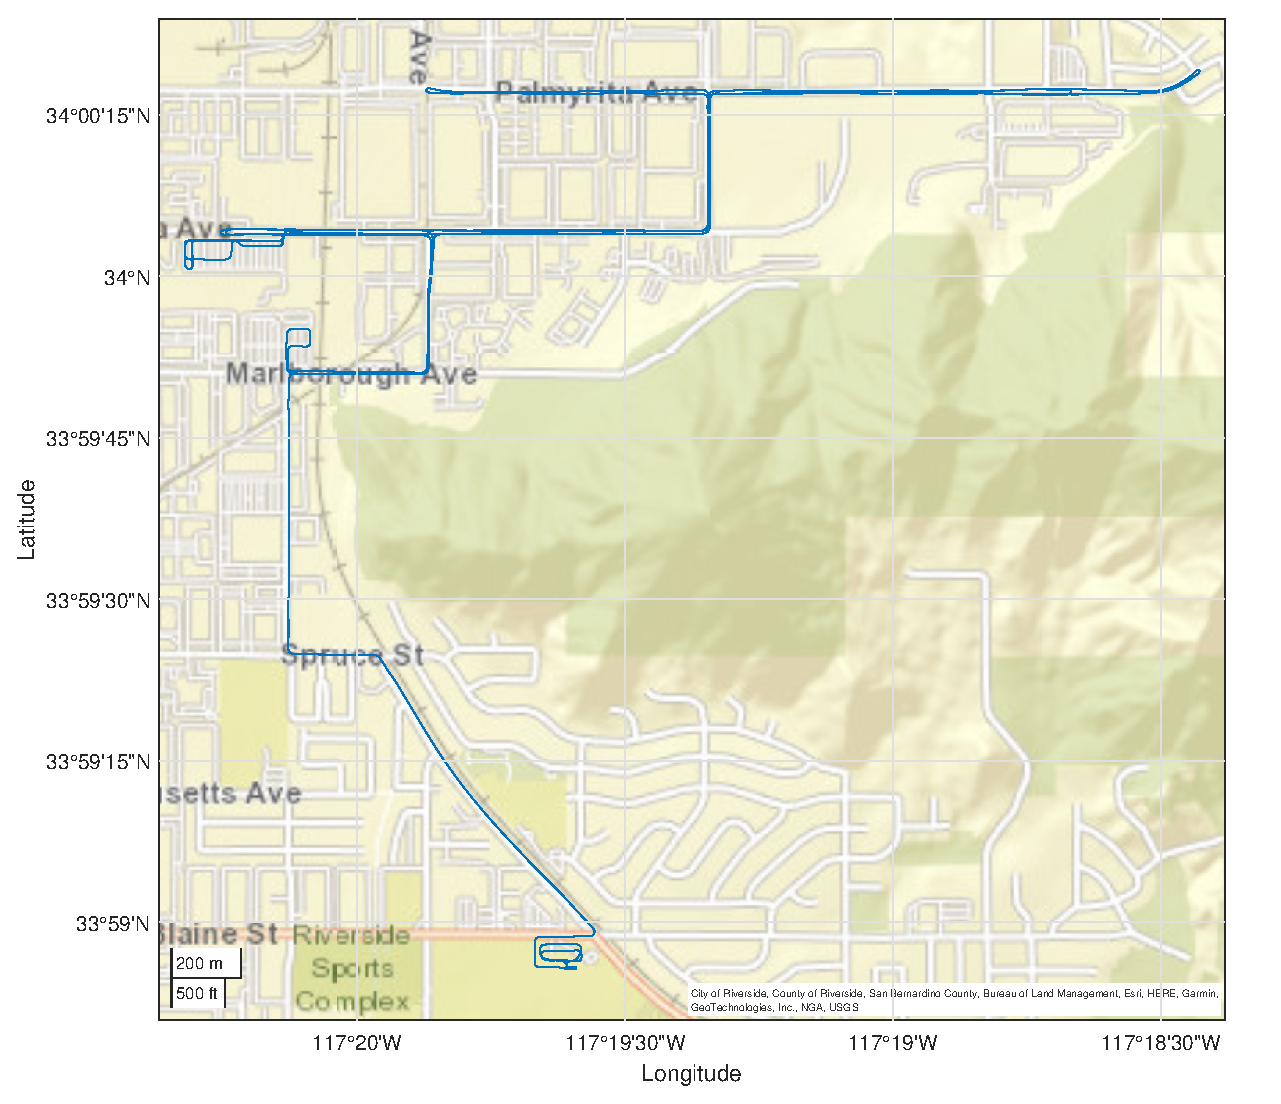
\includegraphics[width=\linewidth]{figures/trajectory_single.eps}
			\caption{Vehicle trajectory for moving test using single band antenna.}
			\label{fig:trj_mt1}
		\end{subfigure}%
		\begin{subfigure}{.5\textwidth}
			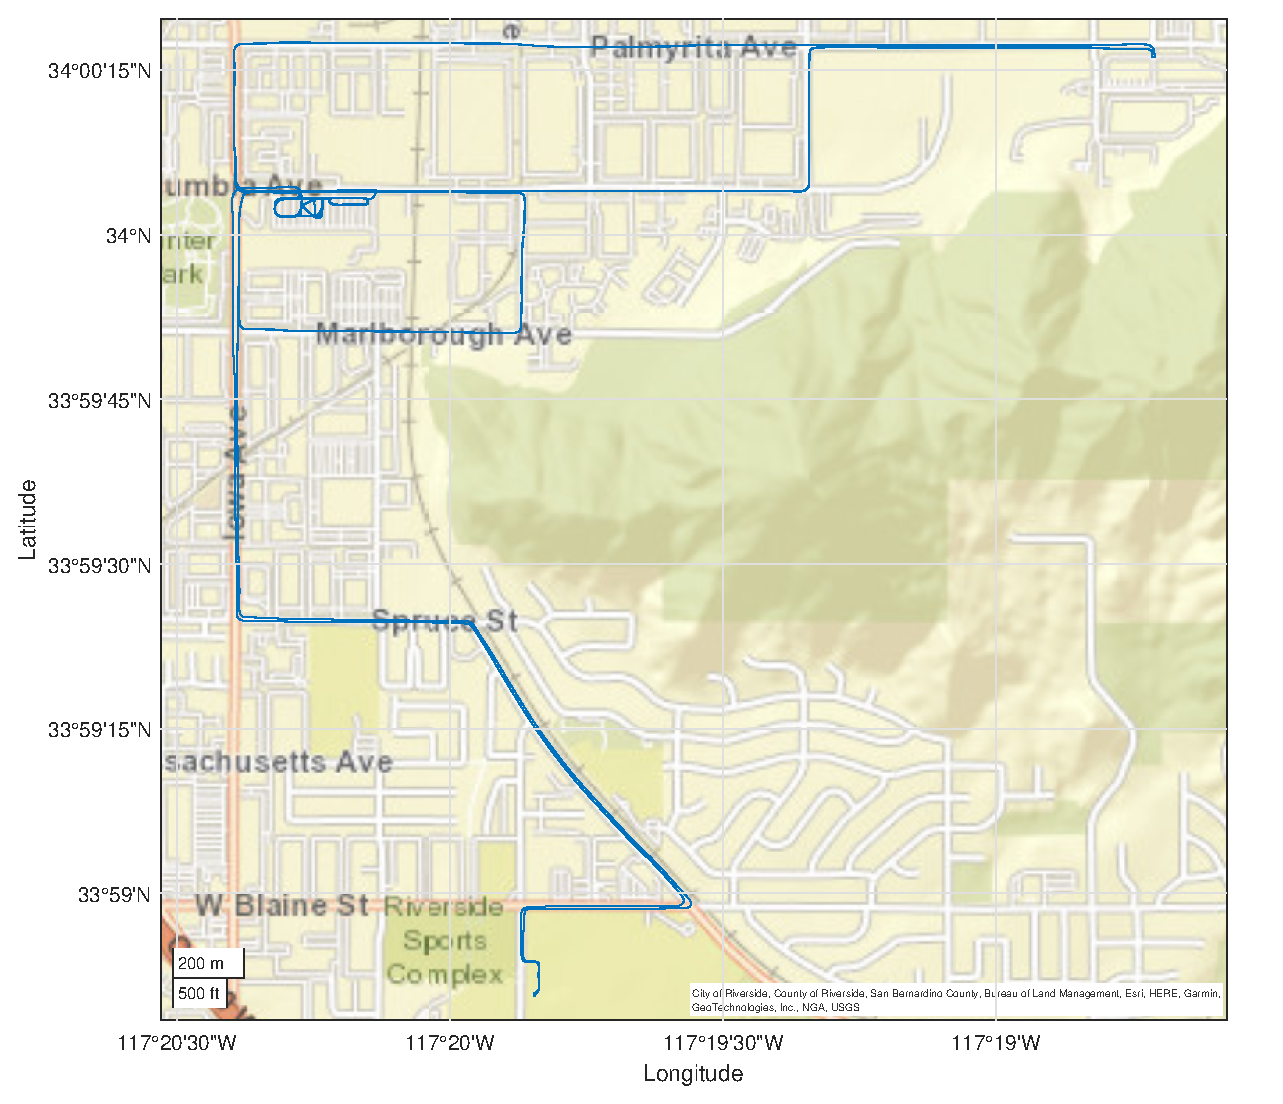
\includegraphics[width=\linewidth]{figures/trajectory_dual.eps}
			\caption{Vehicle trajectory for moving test using dual band antenna.}
			\label{fig:trj_mt2}
		\end{subfigure}
		\caption[short]{Vehicle trajectory for moving test.}
		\label{fig:trj}
	\end{figure}
	
	Fig. \ref{fig:mt1_sky} and Fig. \ref{fig:mt2_sky} show the sky plots with satellite ID at its last destination. Each satellite includes a system symbol and its identifier. `G' stands for GPS, `E' stands for GALILEO, `B' stands for BeiDou. Fig. \ref{fig:mt1_obt} and Fig. \ref{fig:mt2_obt} show more clear satellite orbits without the satellite ID. The green orbit or satellite indicates satellite was used in navigation. The cyan color indicates satellite signal available but not used (In this implementation, they were not used because satellite elevation is lower than elevation cutoff angle). The blue color indicates satellite signal available but not available for use in navigation. The red color indicates satellites signal is not available. Several reasons will cause color blue and red, such as unhealthy status reported by satellite, lack of ephemeris, low signal strength, below elevation cutoff angle setup, and so on \cite{ucenter}. 
	
	Some orbits in both Fig. \ref{fig:mt1} and Fig. \ref{fig:mt2} have different colors shift between available status and unavailable status, such as B21, E5, and G24 in Fig. \ref{fig:mt1}. When the satellites are at low elevation and the vehicle is moving, the receiver may lose tracking of the satellites blocked by high buildings or trees. 
	\begin{figure}[H]
		\centering
		\begin{subfigure}{.45\textwidth}
			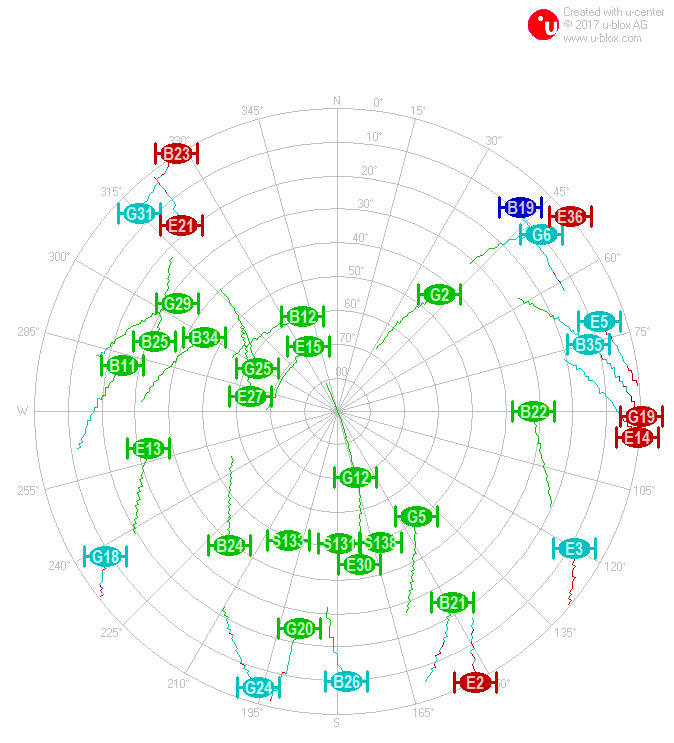
\includegraphics[width=\linewidth]{../Moving_SingleBand/skyplot.png}
			\caption{With satellite ID.}
			\label{fig:mt1_sky}
		\end{subfigure}%
		\begin{subfigure}{.45\textwidth}
			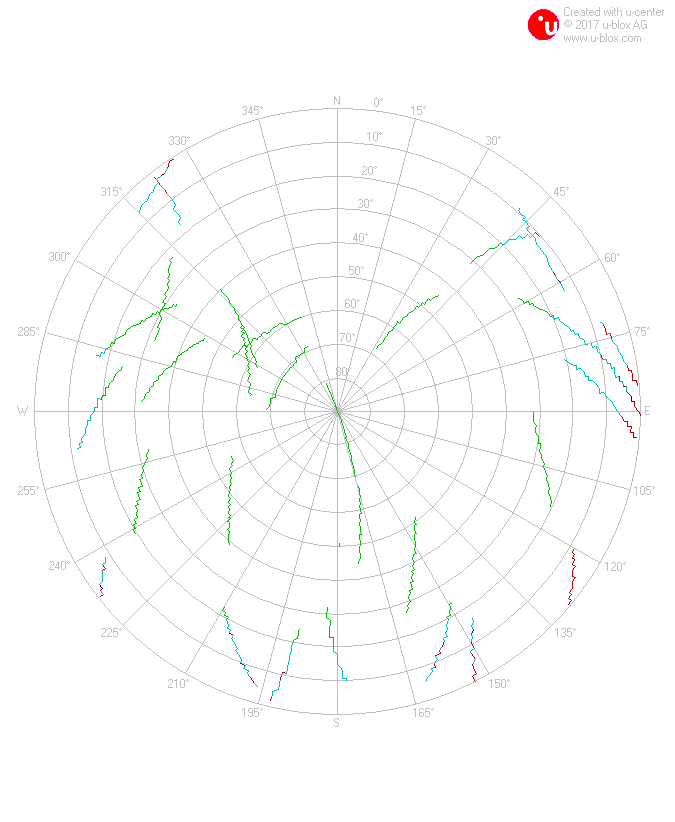
\includegraphics[width=\linewidth]{../Moving_SingleBand/skyplot_orbit.png}
			\caption{	Without satellite ID.}
			\label{fig:mt1_obt}
		\end{subfigure}
		\caption[short]{Sky plot and satellite orbit for moving test using single band antenna.}
		\label{fig:mt1}
	\end{figure}

	\begin{figure}[H]
		\centering
		\begin{subfigure}{.5\textwidth}
			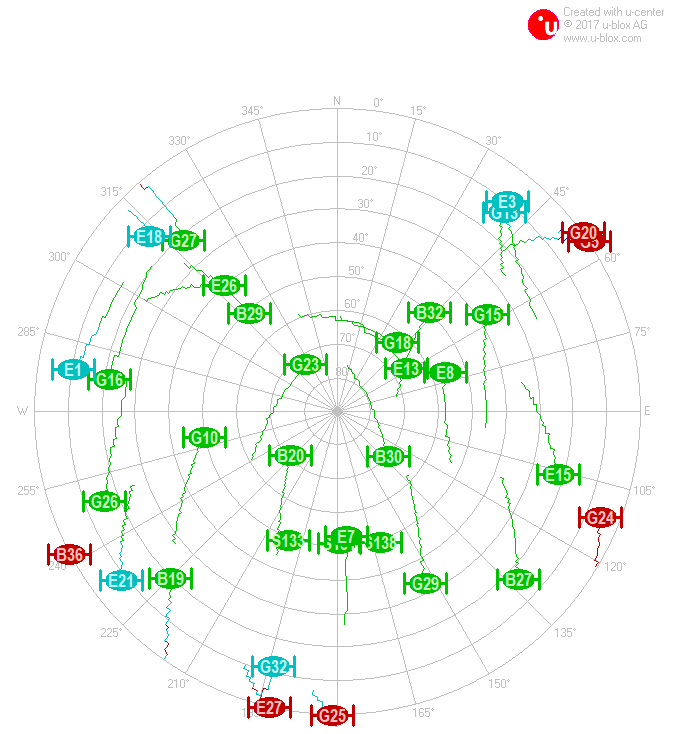
\includegraphics[width=0.9\linewidth]{../Moving_DualBand/skyplot.png}
			\caption{	
				With satellite ID.}
			\label{fig:mt2_sky}
		\end{subfigure}%
		\begin{subfigure}{.5\textwidth}
			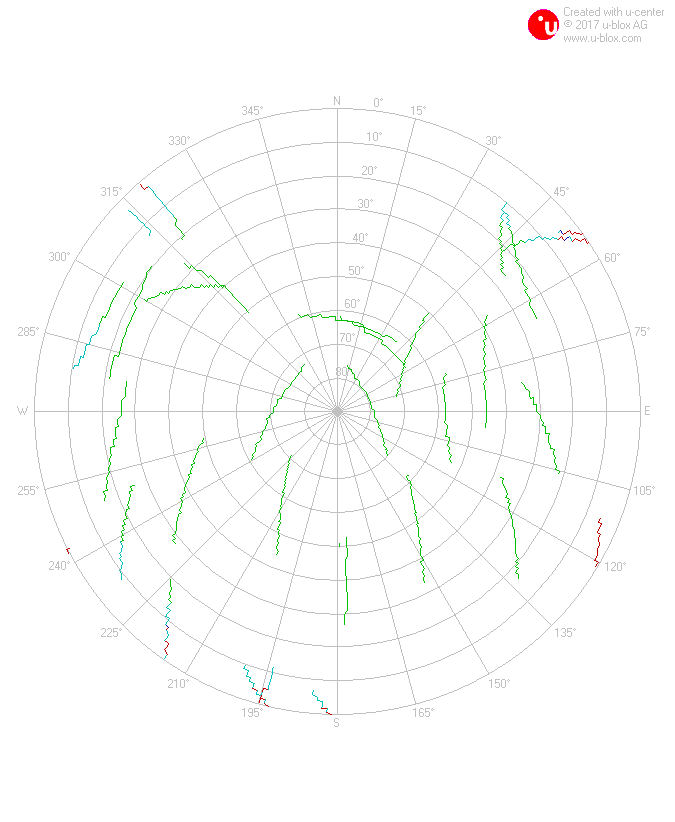
\includegraphics[width=0.9\linewidth]{../Moving_DualBand/skyplot_orbit.png}
			\caption{	
				Without satellite ID.}
			\label{fig:mt2_obt}
		\end{subfigure}
		\caption[short]{Sky plot and satellite orbit for moving test using dual band antenna.}
		\label{fig:mt2}
	\end{figure}
	
	Fig. \ref{fig:m1vspeed}a and Fig. \ref{fig:m2vspeed}a show the horizontal error for the moving test, the analysis can be found in the paper \cite{hu2021using}. Fig. \ref{fig:m1vspeed}b and Fig. \ref{fig:m2vspeed}b show the vehicle speed over ground. Fig. \ref{fig:m1vspeed}c and Fig. \ref{fig:m2vspeed}c show the number of satellites used in navigation. The colors are marked based on the operation used in the experiment, the definition of these acronyms can be founded in Table IV from the paper \cite{hu2021using}. The purple line means the SF GNSS OS, F9P SBAS, SF GNSS VN have the same number of satellites used. These numbers do not count for the SBAS satellites.
	Most cases have the same number but have exceptions which are colored as blue, red, and green. The reason that the number of satellites used suddenly dropped is due to satellite signal loss. The attached video shows an example of the satellite information interface from the u-center from the rerun of moving test for dual-band antenna in F9P SBAS. The column 'Qi' is the signal quality indicator. The description of `Qi' is followed by Table 1. The satellite will be used in pseudorange positioning only when $Qi \geq 4$ which means code locked and time synchronized. In RTK for using carrier data, it requires $Qi = 7$. The `PR used' indicate that if the satellite code measurement is used, Y for yes and N for no. When the satellite signal fades or is blocked by obstructions, such as buildings and trees, the receiver will lose tracking of the signal and the signal quality indicator will be changed to code unlocked statuses ($Qi = 0,1,2,3$). As shown in the video, the Qi of satellite E3 was dropped from 7 to 0 when signal lost, and then back to 7 when the receiver re-lock the satellite. `Qi' change from 7 to other values refers to cycle slip. Cycle slip can be caused by deep rapid signal fading \cite{sennott1992use}. When the receiver detects the cycle slip for a satellite, it will not use this satellite for RTK positioning.
	
	The number of satellites used in RTK is less than others is because the u-blox M8P does not support the GALILEO system.
	
	\begin{table}[H]
		\centering
		\begin{tabular}{|c|c|c|}
			\hline
			Value & Description                                   & Additional remarks                 \\ \hline
			0     & no signal                                     &                                    \\ \hline
			1     & searching signal                              &                                    \\ \hline
			2     & signal acquired                               &                                    \\ \hline
			3     & signal detected but unusable                  &                                    \\ \hline
			4     & code locked and time synchronized             &                                    \\ \hline
			5     & code and carrier locked and time synchronized & carrier lock has not been achieved \\ \hline
			6     & code and carrier locked and time synchronized & carrier lock is intermittent       \\ \hline
			7     & code and carrier locked and time synchronized & carrier lock achieved              \\ \hline
		\end{tabular}
		\label{tab:qi}
		\caption{Definition of signal quality indicator}
	\end{table}
	
	\begin{figure}[H]
		\centering
		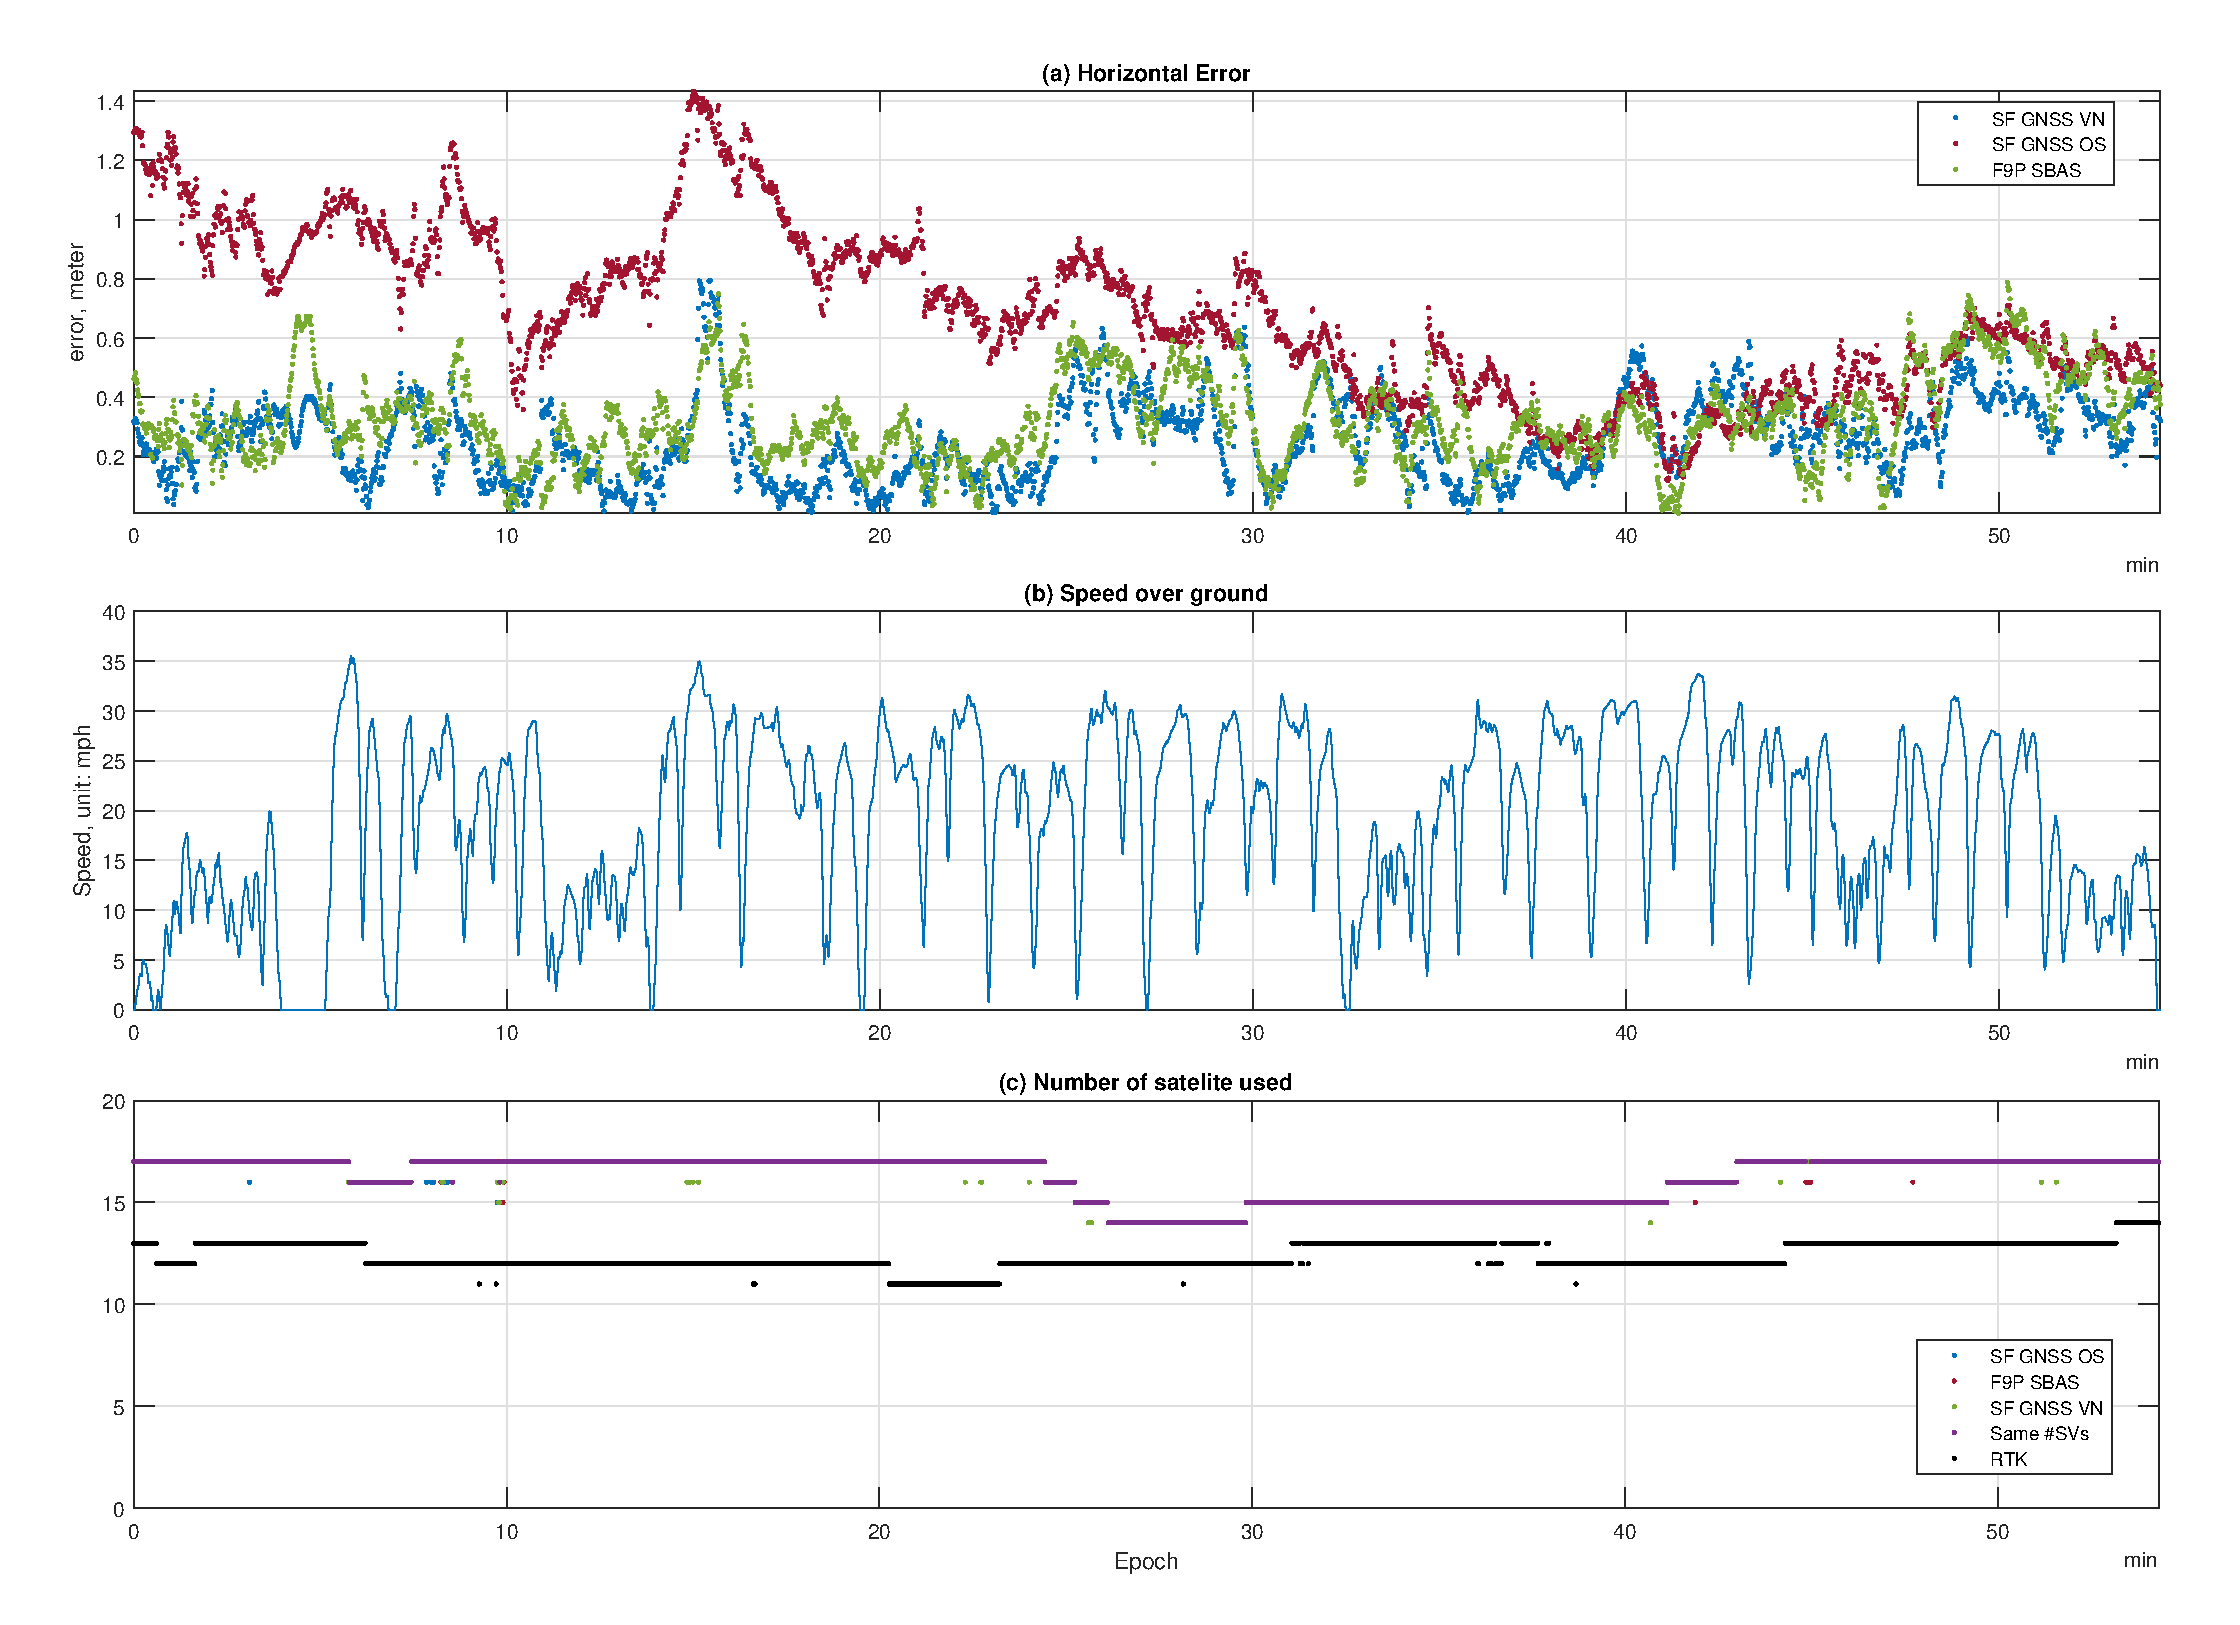
\includegraphics[width=0.9\textwidth]{figures/dynamicinfo_single.eps}
		\caption{Vehicle speed and number of satellites used for moving test using single band antenna.}
		\label{fig:m1vspeed}
	\end{figure}

	\begin{figure}[H]
		\centering
		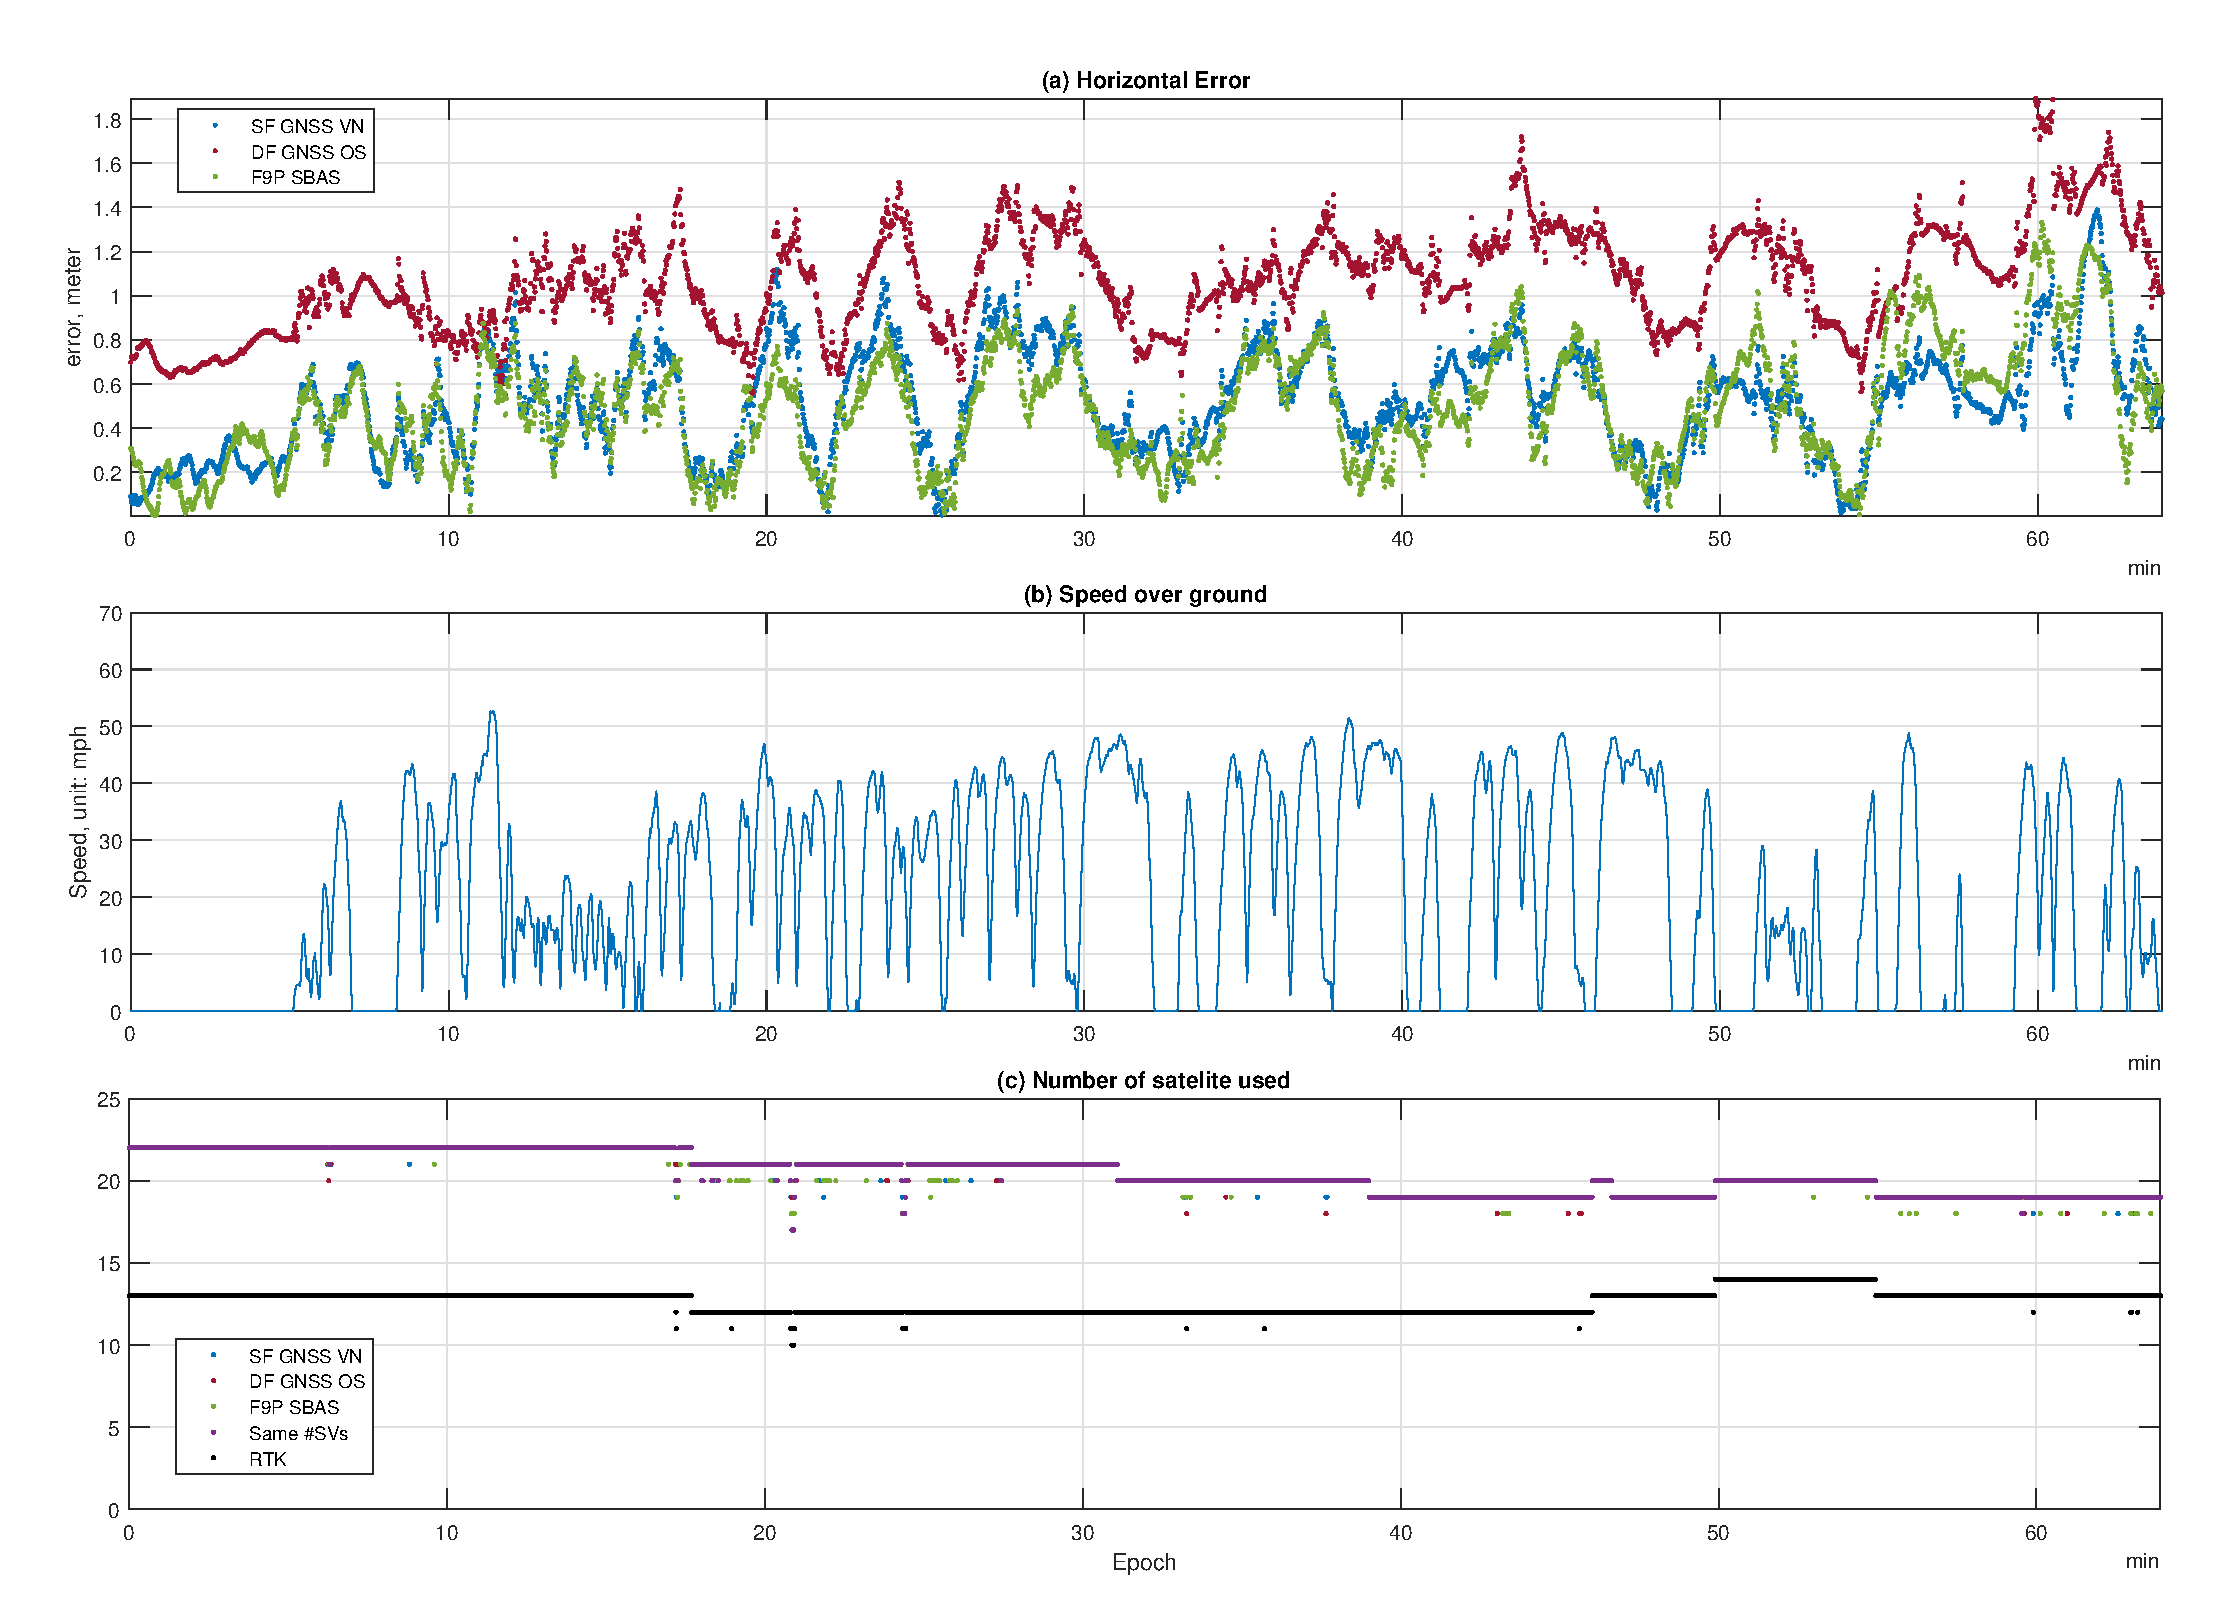
\includegraphics[width=0.9\textwidth]{figures/dynamicinfo_dual.eps}
		\caption{Vehicle speed and number of satellites used for moving test using dual band antenna.}
		\label{fig:m2vspeed}
	\end{figure}

    \bibliographystyle{ieeetr}
    \bibliography{References.bib}

\end{document}